\begin{figure}
  \centering
  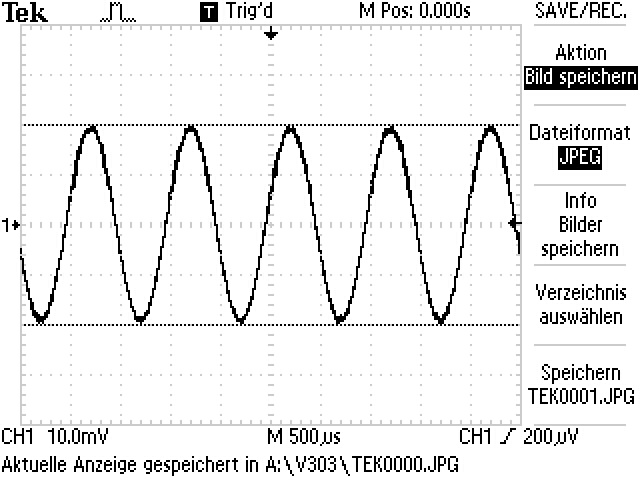
\includegraphics[width=0.8\textwidth]{aufnahmen/eingangssignal.jpg}
  \caption{Vom Funktionsgenerator erzeugte Sinusspannung}
  \label{fig:anfangssignal_ohne_rausch}
\end{figure}

\begin{figure}
  \centering
  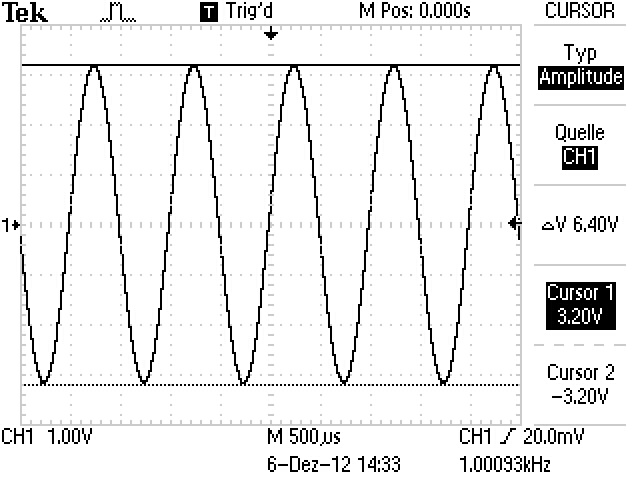
\includegraphics[width=0.8\textwidth]{aufnahmen/referenzsignal.jpg}
  \caption{Vom Funktionsgenerator erzeugtes Referenzsignal}
  \label{fig:referenzsignal_ohne_rausch}
\end{figure}


\begin{figure}
  \centering
  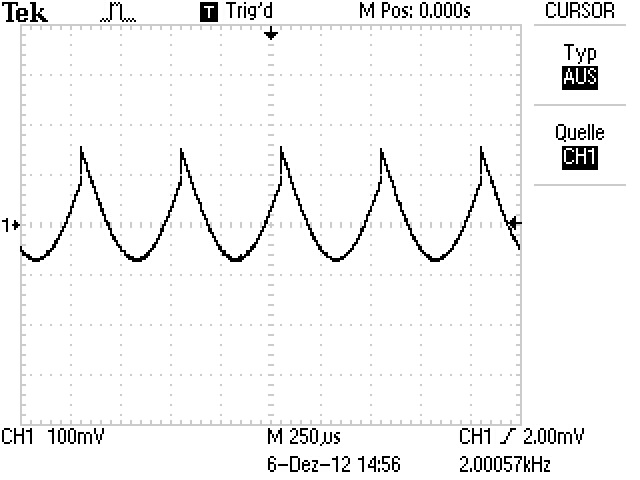
\includegraphics[width=0.8\textwidth]{aufnahmen/phase_0_ohne_rauschen.jpg}
  \caption{Nicht verrauschtes Mischsignal bei eingestellter
    Phasenverschiebung von \SI{0}{\degree}}
    \label{fig:phase_0_nicht_verrauscht}
\end{figure}


\begin{figure}
  \centering
  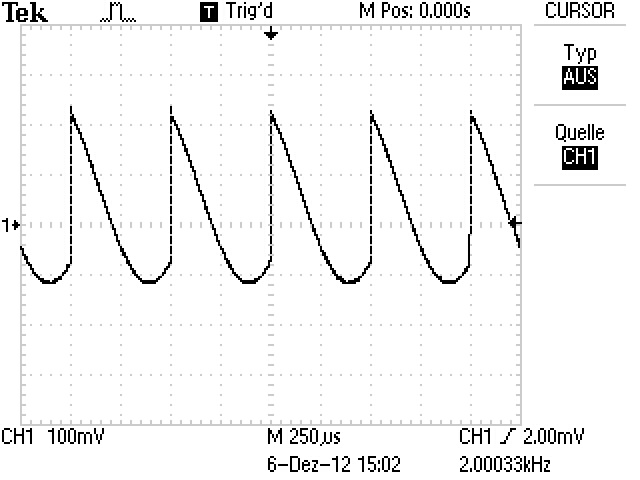
\includegraphics[width=0.8\textwidth]{aufnahmen/phase_45_ohne_rauschen.jpg}
  \caption{Nicht verrauschtes Mischsignal bei eingestellter
    Phasenverschiebung von \SI{45}{\degree}}
  \label{fig:phase_45_nicht_verrauscht}
\end{figure}


\begin{figure}
  \centering
  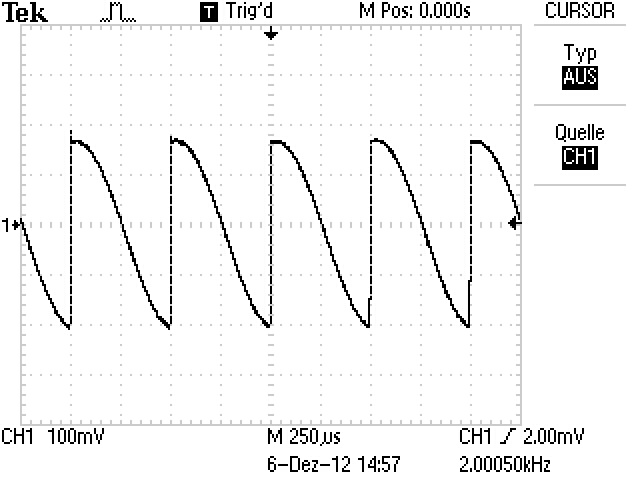
\includegraphics[width=0.8\textwidth]{aufnahmen/phase_90_ohne_rauschen.jpg}
  \caption{Nicht verrauschtes Mischsignal bei eingestellter
    Phasenverschiebung von \SI{90}{\degree}}
  \label{fig:phase_90_nicht_verrauscht}
\end{figure}


\begin{figure}
  \centering
  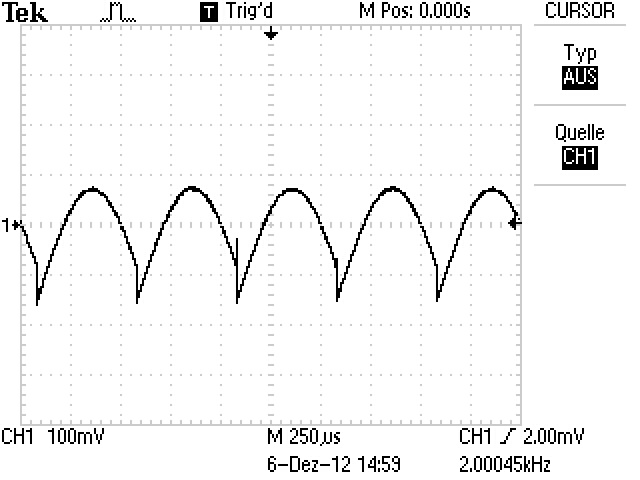
\includegraphics[width=0.8\textwidth]{aufnahmen/phase_180_ohne_rauschen.jpg}
  \caption{Nicht verrauschtes Mischsignal bei eingestellter
    Phasenverschiebung von \SI{180}{\degree}}
  \label{fig:phase_180_nicht_verrauscht}
\end{figure}


\begin{figure}
  \centering
  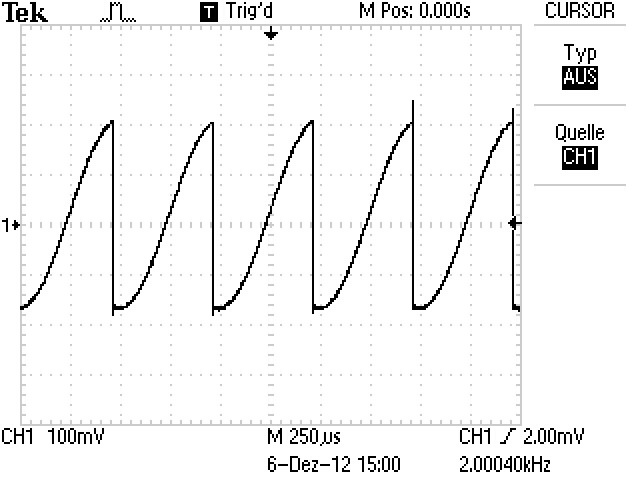
\includegraphics[width=0.8\textwidth]{aufnahmen/phase_270_ohne_rauschen.jpg}
  \caption{Nicht verrauschtes Mischsignal bei eingestellter
    Phasenverschiebung von \SI{270}{\degree}}
  \label{fig:phase_270_nicht_verrauscht}
\end{figure}


\begin{figure}
  \centering
  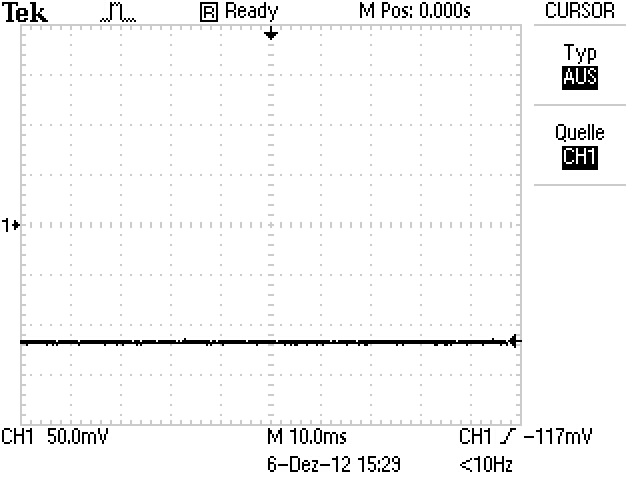
\includegraphics[width=0.8\textwidth]
  {aufnahmen/gleichspannung_ohne_rauschen.jpg}
  \caption{Ausgangssignal des Lock-In-Verstärkers bei nicht verrauschtem
    Eingangssignal}
  \label{fig:gleichspannung_ohne_rausch}
\end{figure}


\begin{figure}
  \centering
  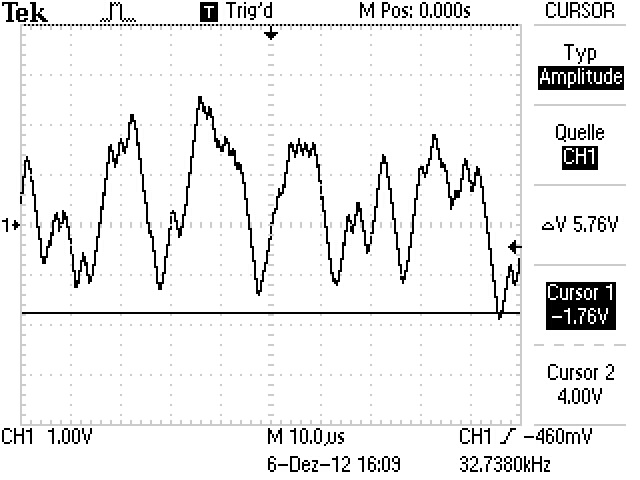
\includegraphics[width=0.8\textwidth]{aufnahmen/vollrausch.jpg}
  \caption{Verrauschtes Eingangssignal}
  \label{fig:vollrausch}
\end{figure}

\begin{figure}
  \centering
  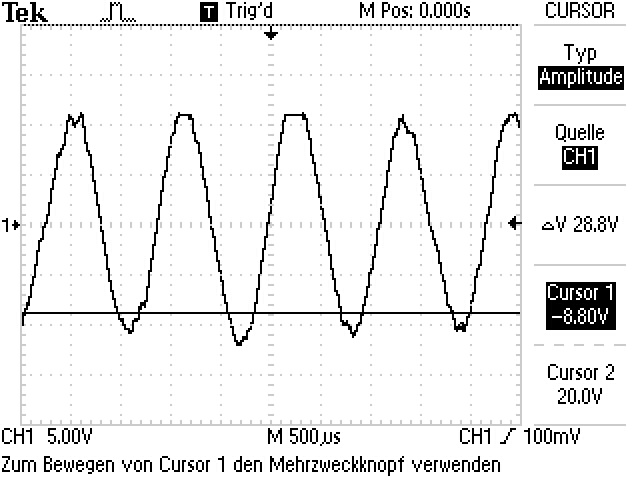
\includegraphics[width=0.8\textwidth]{aufnahmen/bandrausch.jpg}
  \caption{Form des verrauschten Signales nach Bandpassfilter}
  \label{fig:bandrausch}
\end{figure}

\begin{figure}
  \centering
  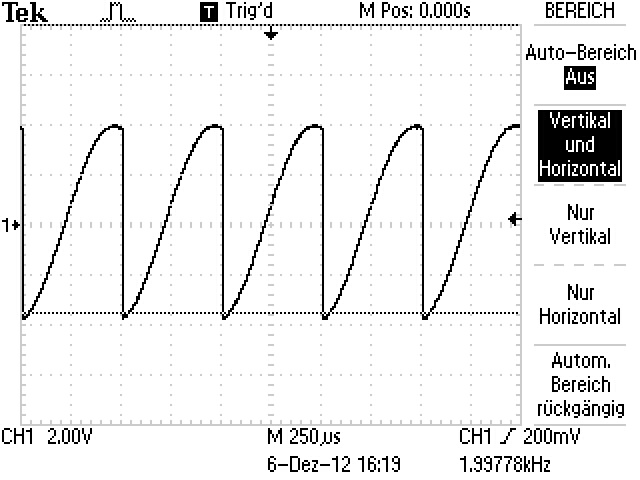
\includegraphics[width=0.8\textwidth]{aufnahmen/phase_0_verrauscht.jpg}
  \caption{Verrauschtes Mischsignal bei eingestellter Phasenverschiebung
    von \SI{0}{\degree}}
  \label{fig:phase_0_verrauscht}
\end{figure}

\begin{figure}
  \centering
  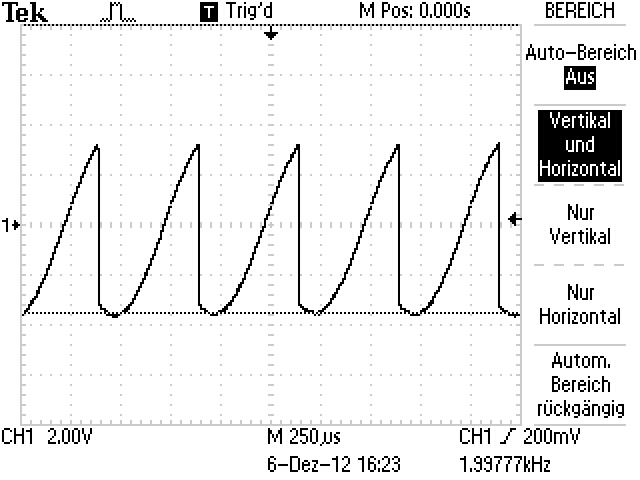
\includegraphics[width=0.8\textwidth]{aufnahmen/phase_45_verrauscht.jpg}
  \caption{Verrauschtes Mischsignal bei eingestellter Phasenverschiebung
    von \SI{45}{\degree}}
  \label{fig:phase_45_verrauscht}
\end{figure}

\begin{figure}
  \centering
  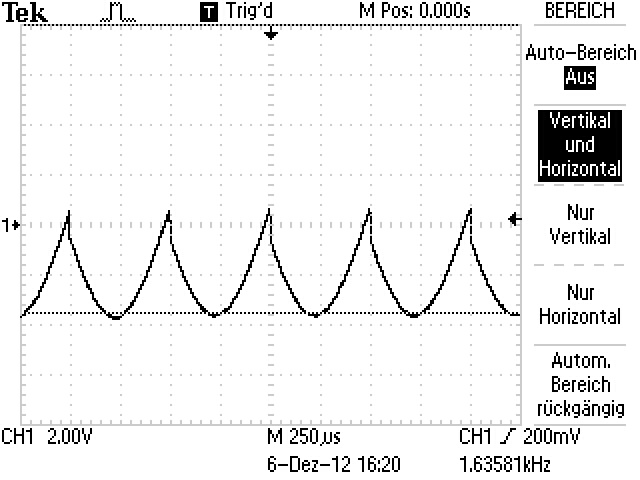
\includegraphics[width=0.8\textwidth]{aufnahmen/phase_90_verrauscht.jpg}
  \caption{Verrauschtes Mischsignal bei eingestellter Phasenverschiebung
    von \SI{90}{\degree}}
  \label{fig:phase_90_verrauscht}
\end{figure}

\begin{figure}
  \centering
  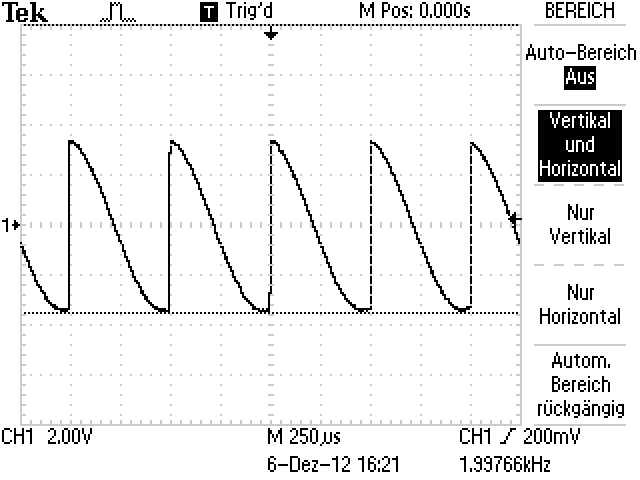
\includegraphics[width=0.8\textwidth]{aufnahmen/phase_180_verrauscht.jpg}
  \caption{Verrauschtes Mischsignal bei eingestellter Phasenverschiebung
    von \SI{180}{\degree}}
  \label{fig:phase_180_verrauscht}
\end{figure}

\begin{figure}
  \centering
  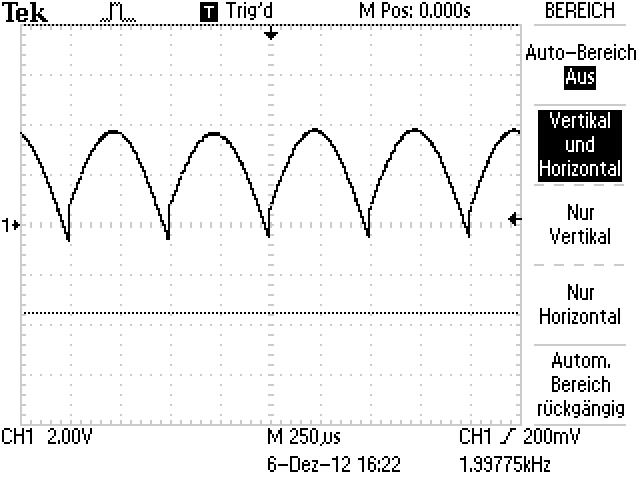
\includegraphics[width=0.8\textwidth]{aufnahmen/phase_270_verrauscht.jpg}
  \caption{Verrauschtes Mischsignal bei eingestellter Phasenverschiebung
    von \SI{270}{\degree}}
  \label{fig:phase_270_verrauscht}
\end{figure}
